\documentclass[tikz,border=8pt]{standalone}
\usepackage{amsmath,amssymb}
\usetikzlibrary{arrows.meta,calc}

\begin{document}
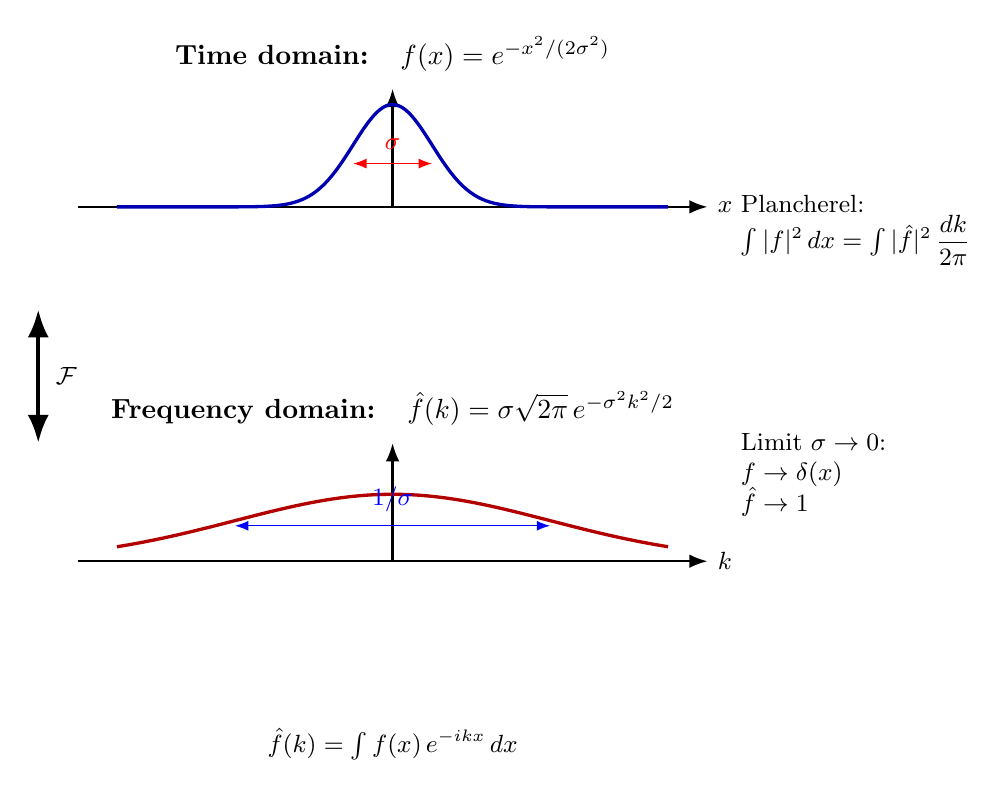
\begin{tikzpicture}[>=Latex]

  % TOP: time/space domain — narrow Gaussian
  \begin{scope}[yshift=3cm]
    \node[font=\bfseries, anchor=south] at (0, 1.6) {Time domain:\quad $f(x)=e^{-x^2/(2\sigma^2)}$};

    \draw[->, thick] (-4.0, 0) -- (4.0, 0) node[right, font=\small]{$x$};
    \draw[->, thick] (0, 0) -- (0, 1.5);

    % sigma=0.5 -> e^{-2 x^2}, narrow
    \draw[blue!70!black, very thick, smooth, samples=140, domain=-3.5:3.5]
      plot(\x, {1.3*exp(-2*\x*\x)});

    \draw[<->, thin, red] (-0.5, 0.55) -- (0.5, 0.55);
    \node[font=\small, red, anchor=south] at (0, 0.6) {$\sigma$};
  \end{scope}

  % Fourier arrow
  \draw[<->, ultra thick] (-4.5, 1.7) -- (-4.5, 0.0);
  \node[font=\small, anchor=west] at (-4.4, 0.85) {$\mathcal F$};

  % BOTTOM: frequency domain — wide Gaussian
  \begin{scope}[yshift=-1.5cm]
    \node[font=\bfseries, anchor=south] at (0, 1.6) {Frequency domain:\quad $\hat f(k)=\sigma\sqrt{2\pi}\,e^{-\sigma^2 k^2/2}$};

    \draw[->, thick] (-4.0, 0) -- (4.0, 0) node[right, font=\small]{$k$};
    \draw[->, thick] (0, 0) -- (0, 1.5);

    % sigma=0.5 -> 1/sigma=2 -> Gaussian width 2, lower amplitude when normalized but here scaled
    \draw[red!70!black, very thick, smooth, samples=140, domain=-3.5:3.5]
      plot(\x, {0.85*exp(-\x*\x/8)});

    \draw[<->, thin, blue] (-2.0, 0.45) -- (2.0, 0.45);
    \node[font=\small, blue, anchor=south] at (0, 0.5) {$1/\sigma$};
  \end{scope}

  % Right side annotations
  \node[font=\small, anchor=west, align=left] at (4.3, 2.7)
    {Plancherel:\\$\int|f|^2\,dx=\int|\hat f|^2\,\dfrac{dk}{2\pi}$};

  \node[font=\small, anchor=west, align=left] at (4.3, -0.4)
    {Limit $\sigma\to 0$:\\$f\to\delta(x)$\\$\hat f\to 1$};

  % bottom main equation
  \node[font=\small, anchor=north] at (0, -3.5)
    {$\hat f(k)=\int f(x)\,e^{-ikx}\,dx$};
\end{tikzpicture}
\end{document}
